%scritto da \PF{}
\subsubsection{UCA 3 - Gestione lista delle organizzazioni}%kite level
\begin{figure}[h!]
	\centering
	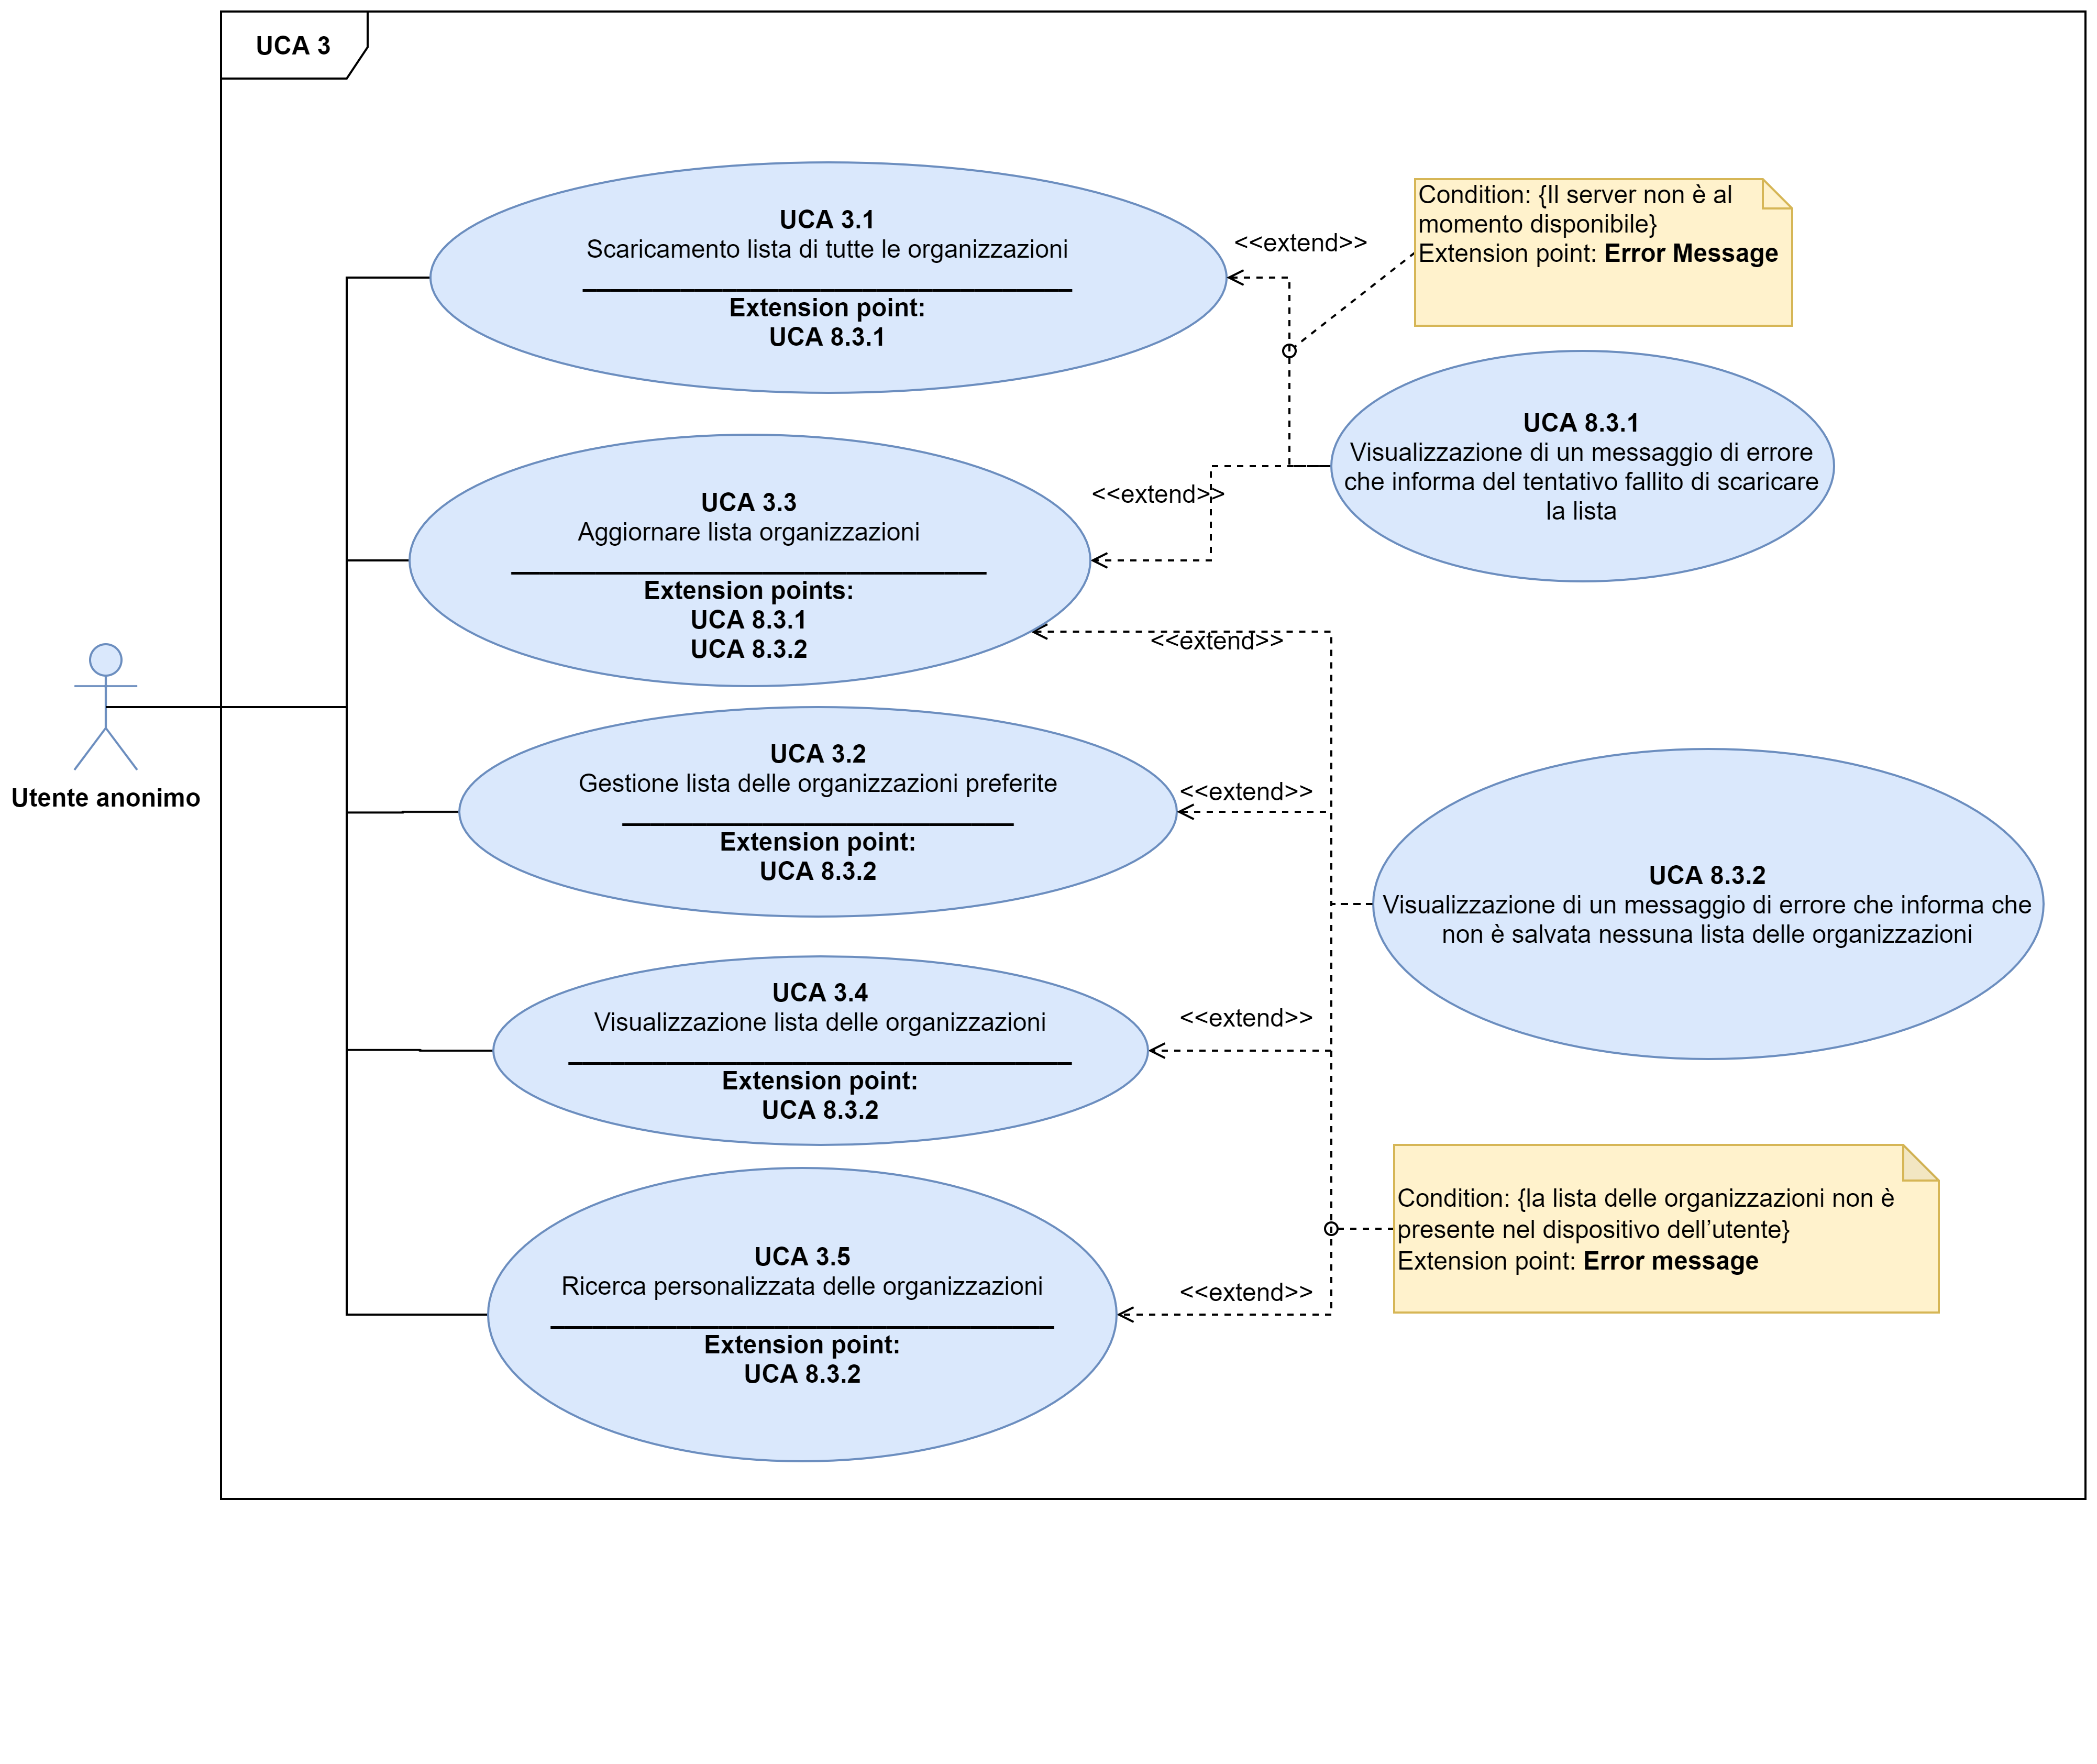
\includegraphics[scale=0.5, center]{Sezioni/UseCase/Immagini/UCA3.png}
	\caption{UCA 3 - Gestione lista delle \glo{organizzazioni}}
\end{figure} 

\begin{itemize}
\item \textbf{Attori primari:} Utente anonimo, Utente riconosciuto
\item \textbf{Precondizione:} L'utente è autenticato e può accedere alle funzionalità della lista delle \glo{organizzazioni}.
\item \textbf{Postcondizione:} Vengono forniti all'utente i risultati delle funzionalità disponibili.
\item \textbf{Scenario principale:} L'utente autenticato utilizza le funzioni di gestione delle liste di \glo{organizzazioni} per svolgere una o più delle seguenti azioni:
	\begin{itemize}
		\item Scaricamento lista di tutte le \glo{organizzazioni} [UCA 3.1];
		\item Gestione lista delle \glo{organizzazioni preferite} [UCA 3.2];
		\item Aggiornare lista \glo{organizzazione} [UCA 3.3];
		\item Visualizzazione lista delle \glo{organizzazioni} [UCA 3.4];
		\item Ricerca personalizzata delle \glo{organizzazioni} [UCA 3.5].
	\end{itemize}
\end{itemize}

\subsubsection{UCA 3.1 - Scaricamento lista di tutte le organizzazioni}%sea level
\begin{itemize}
\item \textbf{Attori primari:} Utente anonimo, Utente riconosciuto
\item \textbf{Precondizione:} L'utente è autenticato e può scaricare la lista di tutte le \glo{organizzazioni}.
\item \textbf{Postcondizione:} L'utente ha a disposizione la lista di tutte le \glo{organizzazioni}.
\item \textbf{Scenario principale:} L'utente seleziona l'esecuzione della funzione "Scaricamento della lista".
\item \textbf{Scenario alternativo:} Se il tentativo di scaricare la lista fallisce viene visualizzato all'utente un messaggio di errore che lo informa di tale problema [UCA 8.3.1].
\item \textbf{Estensioni:}
	\begin{itemize}
	\item UCA 8.3.1 - Visualizzazione di un messaggio di errore che informa del tentativo fallito di scaricare la lista.
\end{itemize}
  
\end{itemize}

\subsubsection{UCA 3.2 - Gestione lista delle organizzazioni preferite}%sea level
\begin{figure}[h]
	\centering
	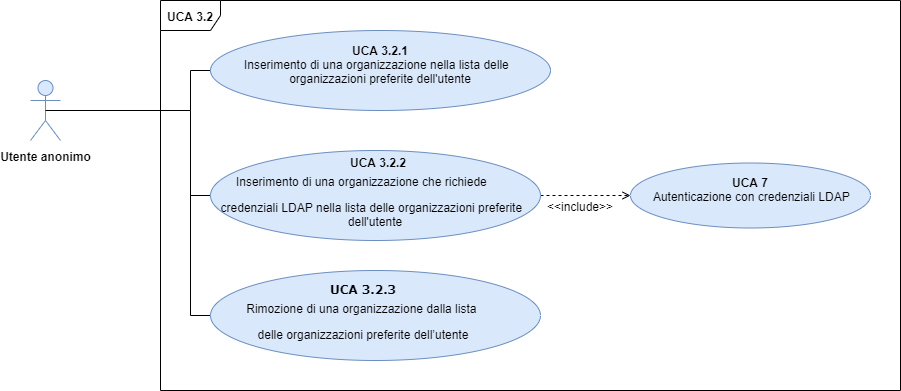
\includegraphics[scale=0.45 , center]{Sezioni/UseCase/Immagini/UCA3.2.png}
	\caption{UCA 3.2 - Gestione lista delle \glo{organizzazioni preferite}}
\end{figure}
\begin{itemize}
	\item \textbf{Attori primari:} Utente anonimo, Utente riconosciuto
	\item \textbf{Precondizione:} L'utente è autenticato e può gestire la propria lista delle \glo{organizzazioni preferite}.
	\item \textbf{Postcondizione:} All'utente vengono forniti i risultati delle funzionalità disponibili.
	\item \textbf{Scenario principale:} L'utente autenticato ha selezionato la funzionalità di gestione della lista delle \glo{organizzazioni preferite}.
	\item \textbf{Flusso di eventi:}
			\begin{enumerate}
			\item L'utente accede alla funzionalità di "Gestioni della lista delle \glo{organizzazioni preferite}";
			\item Vi è la possibilità di inserire un'\glo{organizzazione} nella lista delle \glo{organizzazioni preferite} dell'utente dell'applicazione [UCA 3.2.1], se però viene richiesto di inserire una \glo{organizzazione} che richiede di autenticarsi con credenziali \glo{LDAP} [UCA 3.2.2] allora l'utente dovrà inserire tali credenziali [UCA 7];
			\item Vi è la possibilità di rimuovere un'\glo{organizzazione} dalla lista delle \glo{organizzazioni preferite} dell'utente dell'applicazione [UCA 3.2.3].
			\end{enumerate}
	\item \textbf{Scenario alternativo:} Se non è presente nessuna lista delle \glo{organizzazioni} viene visualizzato all'utente un messaggio di errore che lo informa di tale problema [UCA 8.3.2];
	\item \textbf{Estensioni:}
	\begin{itemize}
		\item UCA 8.3.2 - Visualizzazione di un messaggio di errore che informa che non è salvata nessuna lista delle \glo{organizzazioni}.
	\end{itemize}
	\item \textbf{Inclusioni:}
	\begin{itemize}
			\item UCA 7 - Autenticazione con credenziali LDAP.
	\end{itemize}
\end{itemize}

\subsubsection{UCA 3.2.1 - Inserimento di una organizzazione nella lista delle organizzazioni preferite dell'utente}%fish level
\begin{itemize}
	\item \textbf{Attori primari:} Utente anonimo, Utente riconosciuto
	\item \textbf{Precondizione:} L'utente è autenticato sceglie di eseguire la funzionalità di inserimento di un'\glo{organizzazione} nella lista delle \glo{organizzazioni preferite} (solo se ha scaricato precedentemente la lista delle \glo{organizzazioni}).
	\item \textbf{Postcondizione:} È stata inserita un'\glo{organizzazione} che non richiede tracciamento autenticato, scelta dall'utente, nella lista delle \glo{organizzazioni preferite}.
	\item \textbf{Scenario principale:} Inserimento di una organizzazione che non richiede tracciamento autenticato nella lista delle organizzazioni preferite dell'utente.
	\item \textbf{Flusso di eventi:}
	\begin{enumerate}
		\item L'utente seleziona dalla lista delle \glo{organizzazioni} l'\glo{organizzazione}, la quale non richiede tracciamento autenticato, da inserire nella lista delle \glo{organizzazioni preferite};
		\item L'utente conferma l'inserimento nella lista delle \glo{organizzazioni preferite} per l'\glo{organizzazione} scelta.
	\end{enumerate}
\end{itemize}

\subsubsection{UCA 3.2.2 - Inserimento di una organizzazione che richiede credenziali LDAP nella lista delle organizzazioni preferite dell'utente}%fish level
\begin{itemize}
	\item \textbf{Attori primari:} Utente anonimo, Utente riconosciuto
	\item \textbf{Precondizione:} L'utente è autenticato e sceglie di eseguire la funzionalità di inserimento nella lista delle \glo{organizzazioni preferite} solo se ha scaricato precedentemente la lista delle \glo{organizzazioni}.
	\item \textbf{Postcondizione:} È stata inserita un'\glo{organizzazione}, che richiede tracciamento autenticato, scelta dall'utente, nella lista delle \glo{organizzazioni preferite}.
	\item \textbf{Scenario principale:} Inserimento di una organizzazione con tracciamento autenticato nella lista delle organizzazioni preferite dell'utente.
	\item \textbf{Flusso di eventi:}
	\begin{enumerate}
		\item L'utente seleziona dalla lista delle \glo{organizzazioni} l'\glo{organizzazione}, la quale richiede tracciamento autenticato, da inserire nella lista delle \glo{organizzazioni preferite};
		\item L'utente conferma l'inserimento nella lista delle \glo{organizzazioni preferite} per l'\glo{organizzazione} scelta;
		\item L'utente si autentica con credenziali \glo{LDAP} [UCA 7].
	\end{enumerate}
	\item \textbf{Inclusioni:}
	\begin{itemize}
			\item UCA 7 - Autenticazione con credenziali LDAP.
	\end{itemize}
\end{itemize}

\subsubsection{UCA 3.2.3 - Rimozione di una organizzazione dalla lista delle organizzazioni preferite dell'utente}%fish level
\begin{itemize}
	\item \textbf{Attori primari:} Utente anonimo, Utente riconosciuto
	\item \textbf{Precondizione:}  L'utente è autenticato sceglie di eseguire la funzionalità di rimozione nella lista delle \glo{organizzazioni preferite} solo se c'è almeno una \glo{organizzazione} inserita nella lista delle \glo{organizzazioni preferite}.
	\item \textbf{Postcondizione:} È stata rimossa l'\glo{organizzazione}, scelta dall'utente, dalla lista delle \glo{organizzazioni preferite}.
	\item \textbf{Scenario principale:} Rimozione di una organizzazione dalla lista delle organizzazioni preferite dell'utente.
	\item \textbf{Flusso di eventi:}
	\begin{enumerate}
		\item L'utente seleziona nella lista delle \glo{organizzazioni preferite} l'\glo{organizzazione} da rimuovere dalla lista delle \glo{organizzazioni preferite};
		\item L'utente conferma la rimozione dalla lista delle \glo{organizzazioni preferite} per l'\glo{organizzazione} scelta.
	\end{enumerate}
\end{itemize}

\subsubsection{UCA 3.3 - Aggiornare lista organizzazioni}%sea level

\begin{figure}[h]
	\centering
	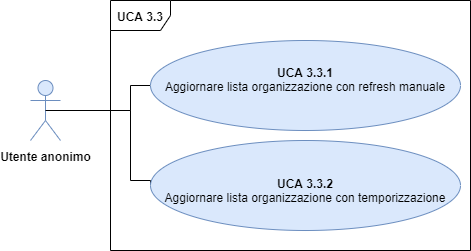
\includegraphics[scale=0.5, center]{Sezioni/UseCase/Immagini/UCA3.3.png}
	\caption{UCA 3.3 - Aggiornare lista \glo{organizzazioni}}
\end{figure}

\begin{itemize} 
	\item \textbf{Attori primari:} Utente anonimo, Utente riconosciuto
	\item \textbf{Precondizione:} L'utente è autenticato e può aggiornare la lista delle \glo{organizzazioni}.
	\item \textbf{Postcondizione:} L'utente ha aggiornato la lista di tutte le \glo{organizzazioni}.
	\item \textbf{Scenario principale:} L'utente ha la necessità di aggiornare la lista e può farlo manualmente con l'apposita funzionalità [UCA 3.3.1] o sarà fatto con temporizzazione [UCA 3.3.2].
	\item \textbf{Scenario alternativo 1:} Se il tentativo di scaricare la lista fallisce viene visualizzato all'utente un messaggio di errore che lo informa di tale problema [UCA 8.3.1].
	\item \textbf{Scenario alternativo 2:} Se non è presente nessuna lista delle \glo{organizzazioni} viene visualizzato all'utente un messaggio di errore che lo informa di tale problema [UCA 8.3.2];
	\item \textbf{Estensioni:}
	\begin{itemize}
		\item UCA 8.3.1 - Visualizzazione di un messaggio di errore che informa del tentativo fallito di scaricare la lista;
		\item UCA 8.3.2 - Visualizzazione di un messaggio di errore che informa che non è salvata nessuna lista delle \glo{organizzazioni}.
	\end{itemize}
\end{itemize}

\subsubsection{UCA 3.3.1 - Aggiornare lista organizzazione con refresh manuale}%fish level
\begin{itemize}
	\item \textbf{Attori primari:} Utente anonimo, Utente riconosciuto
	\item \textbf{Precondizione:} L'utente anonimo sceglie di eseguire la funzionalità aggiornamento della lista dell'\glo{organizzazione} attraverso la modalità di \glo{refresh manuale}.
	\item \textbf{Postcondizione:} La lista delle \glo{organizzazioni} è aggiornata.	
	\item \textbf{Scenario principale:} Aggiornamento della lista delle organizzazione con il refresh manuale.
	\item \textbf{Generalizzazione:}
	\begin{enumerate}
	\item UCA 3.3 - Aggiornare lista organizzazioni.
	\end{enumerate}
\end{itemize}

\subsubsection{UCA 3.3.2 - Aggiornare lista organizzazione con temporizzazione}%fish level
\begin{itemize} 
	\item \textbf{Attori primari:} Utente anonimo, Utente riconosciuto
	\item \textbf{Precondizione:} L'utente anonimo sceglie di eseguire la funzionalità aggiornamento della lista dell'\glo{organizzazione} attraverso la modalità \glo{temporizzazione}.
	\item \textbf{Postcondizione:} La lista delle \glo{organizzazioni} è aggiornata.
	\item \textbf{Scenario principale:} Aggiornamento della lista delle organizzazione con temporizzazione.
	\item \textbf{Generalizzazione:}
	\begin{enumerate}
	\item UCA 3.3 - Aggiornare lista organizzazioni.
	\end{enumerate}	
\end{itemize}

\subsubsection{UCA 3.4 - Visualizzazione lista delle organizzazioni}%sea level

\begin{figure}[h]
	\centering	
	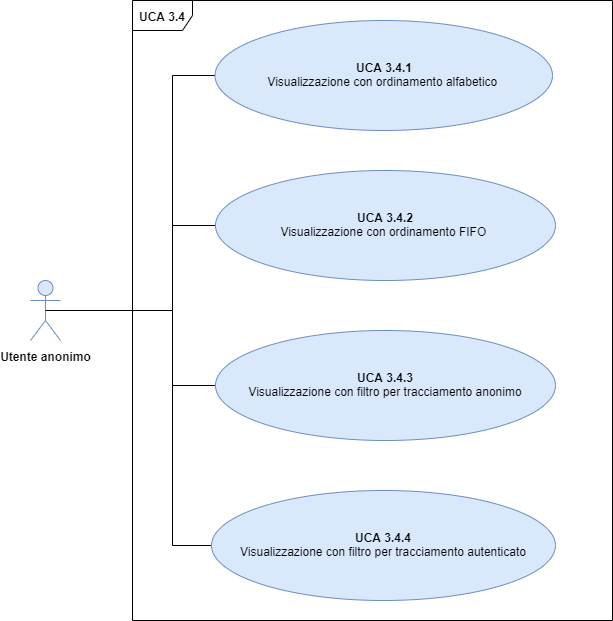
\includegraphics[scale=0.45, center]{Sezioni/UseCase/Immagini/UCA3.4.png}
	\caption{UCA 3.4 - Visualizzazione lista delle \glo{organizzazioni}}
\end{figure}

\begin{itemize} 
	\item \textbf{Attori primari:} Utente anonimo, Utente riconosciuto
	\item \textbf{Precondizione:}  L'utente è autenticato e può visualizzare la lista delle \glo{organizzazioni}.
	\item \textbf{Postcondizione:} L'utente visualizza la lista delle \glo{organizzazioni} nel modo che ritiene più opportuno.
	\item \textbf{Scenario principale:}	L'utente può scegliere come visualizzare la lista tramite diversi tipi di ordinamento:
	\begin{enumerate}
		\item Visualizzazione con ordinamento alfabetico [UCA 3.4.1];
		\item Visualizzazione con ordinamento \glo{FIFO} [UCA 3.4.2];
	\end{enumerate}
	\item \textbf{Scenario alternativo:} Se non è presente nessuna lista delle \glo{organizzazioni} viene visualizzato all'utente un messaggio di errore che lo informa di tale problema.
	\item \textbf{Estensioni:}
	\begin{itemize}
		\item UCA 8.3.2 - Visualizzazione di un messaggio di errore che informa che non è salvata nessuna lista delle organizzazioni.
	\end{itemize}
\end{itemize}

\subsubsection{UCA 3.4.1 - Visualizzazione con ordinamento alfabetico}%fish level
\begin{itemize}
	\item \textbf{Attori primari:} Utente anonimo, Utente riconosciuto
	\item \textbf{Precondizione:} L'utente autenticato può utilizzare la funzionalità di visualizzazione della lista secondo un ordinamento alfabetico (dalla a alla z) per il nome dell'\glo{organizzazione}.
	\item \textbf{Postcondizione:} Viene visualizzata la lista delle \glo{organizzazioni} in ordine alfabetico per il nome dell'\glo{organizzazione}.
	\item \textbf{Scenario principale:} Visualizzazione della lista delle organizzazioni con ordinamento alfabetico.
	\item \textbf{Generalizzazione:}
	\begin{enumerate}
	\item UCA 3.4 - Visualizzazione lista delle organizzazioni.
	\end{enumerate}	
\end{itemize}

\subsubsection{UCA 3.4.2 - Visualizzazione con ordinamento \glo{FIFO}}%fish level
\begin{itemize}	
	\item \textbf{Attori primari:} Utente anonimo, Utente riconosciuto
	\item \textbf{Precondizione:} L'utente autenticato può utilizzare la funzionalità di visualizzazione della lista secondo un ordinamento \glo{FIFO}.
	\item \textbf{Postcondizione:} Viene visualizzato la lista delle \glo{organizzazioni} secondo un ordinamento \glo{FIFO}.
	\item \textbf{Scenario principale:} Visualizzazione della lista delle organizzazioni con ordinamento \glo{FIFO}.
	\item \textbf{Generalizzazione:}
	\begin{enumerate}
	\item UCA 3.4 - Visualizzazione lista delle organizzazioni.
	\end{enumerate}	
\end{itemize}


\subsubsection{UCA 3.5 - Ricerca personalizzata delle organizzazioni}%sea level
\begin{figure}[h]
	\centering
	
	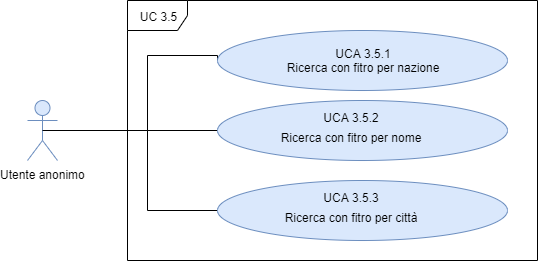
\includegraphics[scale=0.5, center]{Sezioni/UseCase/Immagini/UCA3.5.png}
	\caption{UCA 3.5 - Ricerca personalizzata delle \glo{organizzazioni}}
\end{figure}
\begin{itemize}
	\item \textbf{Attori primari:} Utente anonimo, Utente riconosciuto
	\item \textbf{Precondizione:} L'utente è autenticato e può svolgere ricerche riguardo le \glo{organizzazioni}.
	\item \textbf{Postcondizione:} Vengono forniti all'utente i risultati delle ricerche.
	\item \textbf{Scenario principale:} L'utente deve svolgere alcune ricerche e sceglie il metodo che più lo aggrada.
	\item \textbf{Flusso di eventi:} 
	\begin{enumerate}
		\item L'utente anonimo accede alla funzionalità di ricerca personalizzata della lista delle \glo{organizzazioni} per ricercare le \glo{organizzazioni} desiderate;
		\item L'utente ha la possibilità di effettuare la ricerca per nazione [UCA 3.5.1];
		\item L'utente ha la possibilità di effettuare la ricerca per nome [UCA 3.5.2];
		\item L'utente ha la possibilità di effettuare la ricerca per città [UCA 3.5.3].
	\end{enumerate}
	\item \textbf{Scenario alternativo:} Se non è presente nessuna lista delle \glo{organizzazioni} viene visualizzato all'utente un messaggio di errore che lo informa di tale problema [UCA 8.3.2].
	\item \textbf{Estensioni:}
	\begin{itemize}
		\item UCA 8.3.2 - Visualizzazione di un messaggio di errore che informa che non è salvata nessuna lista delle organizzazioni.
	\end{itemize}
\end{itemize}

\subsubsection{UCA 3.5.1 - Ricerca con filtro per nazione}%fish level
\begin{itemize}
	\item \textbf{Attori primari:} Utente anonimo, Utente riconosciuto
	\item \textbf{Precondizione:} L'utente autenticato può utilizzare la funzionalità di ricerca della lista per cercare le \glo{organizzazioni} di una certa nazione d'interesse.
	\item \textbf{Postcondizione:} Viene visualizzato la lista delle \glo{organizzazioni} che sono nella nazione scelta dall'utente.
	\item \textbf{Scenario principale:} Le ricerche vengono effettuate tramite un filtro per nazione.
	\item \textbf{Generalizzazione:}
	\begin{enumerate}
	\item UCA 3.5 - Ricerca personalizzata delle organizzazioni.
	\end{enumerate}	
\end{itemize}

\subsubsection{UCA 3.5.2 - Ricerca con filtro per nome}%fish level
\begin{itemize}
	\item \textbf{Attori primari:} Utente anonimo, Utente riconosciuto
	\item \textbf{Precondizione:} L'utente autenticato può utilizzare la funzionalità di ricerca della lista per cercare le \glo{organizzazioni} che hanno nel nome una sottostringa specificata dall'utente.
	\item \textbf{Postcondizione:} Viene visualizzato la lista delle \glo{organizzazioni} che hanno nel nome una sottostringa scelta dall'utente.
	\item \textbf{Scenario principale:} Le ricerche vengono effettuate tramite un filtro per nome.
	\item \textbf{Generalizzazione:}
	\begin{enumerate}
	\item UCA 3.5 - Ricerca personalizzata delle organizzazioni.
	\end{enumerate}	
\end{itemize}

\subsubsection{UCA 3.5.3 - Ricerca con filtro per città}%fish level
\begin{itemize}
	\item \textbf{Attori primari:} Utente anonimo, Utente riconosciuto
	\item \textbf{Precondizione:} L'utente autenticato può utilizzare la funzionalità di ricerca della lista per cercare le \glo{organizzazioni} di una certa città d'interesse.
	\item \textbf{Postcondizione:} Viene visualizzato la lista delle \glo{organizzazioni} che sono nella città scelta dall'utente.
	\item \textbf{Scenario principale:} Le ricerche vengono effettuate tramite un filtro per città.
	\item \textbf{Generalizzazione:}
	\begin{enumerate}
	\item UCA 3.5 - Ricerca personalizzata delle organizzazioni.
	\end{enumerate}	
\end{itemize}

\subsubsection{UCA 3.5.4 - Visualizzazione con filtro per tracciamento anonimo}%fish level
\begin{itemize}
	\item \textbf{Attori primari:} Utente anonimo, Utente riconosciuto
	\item \textbf{Precondizione:} L'utente autenticato può utilizzare la funzionalità di visualizzazione della lista che permettono un \glo{tracciamento anonimo}.
	\item \textbf{Postcondizione:} Viene visualizzato la lista delle \glo{organizzazioni} che richiedono il \glo{tracciamento anonimo}.
	\item \textbf{Scenario principale:} Visualizzazione della lista delle organizzazioni con filtro per tracciamento anonimo.
	\item \textbf{Generalizzazione:}
	\begin{enumerate}
	\item UCA 3.5 - Ricerca personalizzata delle organizzazioni.
	\end{enumerate}	
\end{itemize}

\subsubsection{UCA 3.5.5 - Visualizzazione con filtro per \glo{tracciamento autenticato}}%fish level
\begin{itemize}
	\item \textbf{Attori primari:} Utente anonimo, Utente riconosciuto
	\item \textbf{Precondizione:} L'utente autenticato può utilizzare la funzionalità di visualizzazione della lista che permette un \glo{tracciamento autenticato}.
	\item \textbf{Postcondizione:} Viene visualizzato la lista delle \glo{organizzazioni} che permettono il \glo{tracciamento autenticato}.
	\item \textbf{Scenario principale:} Visualizzazione della lista delle organizzazioni con filtro per \glo{tracciamento autenticato}.
	\item \textbf{Generalizzazione:}
	\begin{enumerate}
	\item UCA 3.5 - Ricerca personalizzata delle organizzazioni.
	\end{enumerate}	
\end{itemize}